\section{Preliminaries and related work}
\subsection{Definitions and conventions}
Let $G=(V,E)$ be a finite simple undirected graph, and let
$D_2=\{\{u,v\}:d_G(u,v)=2\}$ contain unordered vertex pairs at shortest-path
distance exactly two. For integers $h\geq k\geq1$, a labeling
$f:V\to\mathbb Z_{\geq0}$ satisfies
\[
 |f(u)-f(v)|\geq h\quad(\{u,v\}\in E),\qquad
 |f(u)-f(v)|\geq k\quad(\{u,v\}\in D_2).
\]
Its span is $\max_v f(v)-\min_v f(v)$; the minimum span is
$\lambda_{h,k}(G)$. Translating the minimum label to zero preserves every
constraint. Thus a decision test for span at most $s$ uses labels
$0,\ldots,s$, with $s+1$ available values. Vertices farther than two apart
may share a label. Disconnected components impose no constraints on one
another, and their optimal spans combine by taking the maximum. An empty
or edgeless graph has span zero.


For a nonempty graph, its square $G^2$ joins vertices at distance one or
two in $G$. In particular,
\[
 \lambda_{1,1}(G)=\chi(G^2)-1.
\]
A proper coloring with $q$ colors yields labels $0,\ldots,q-1$;
conversely, integer labels of span $s$ use at most $s+1$ colors of $G^2$.
This connects the equal-parameter case to coloring without identifying
arbitrary $L(h,k)$ instances with ordinary coloring.

We write $P_n,C_n$ for paths and cycles. The Cartesian product
$G\square H$ has vertices $(u,v)$; an edge changes exactly one coordinate
along an edge of that factor. The corona $G\circ H$ attaches a separate
copy of $H$ to every vertex of $G$, adjacent to all vertices in its copy.
For $|V(G)|=n$ and $|V(H)|=m$, the corona has $n(m+1)$ vertices.
Figure~\ref{fig:submission-labeling} illustrates labels and thresholds.

\begin{figure}[htbp]
\centering
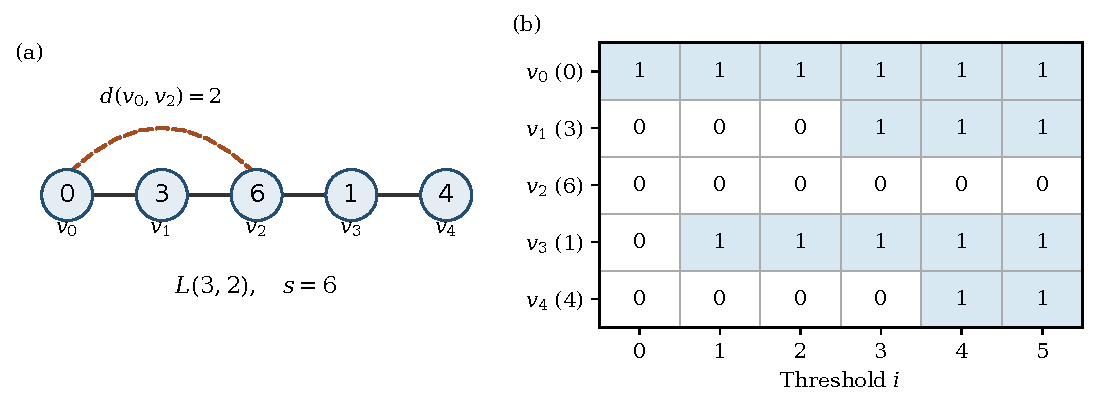
\includegraphics[width=\linewidth]{paper/generated/manuscript_figures/labeling_order.pdf}
\caption{A labeling and its threshold representation.}
\label{fig:submission-labeling}
\tablenote{The labels $0,3,6,1,4$ on $P_5$ satisfy $L(3,2)$ and have
span 6. The dashed arc indicates a distance-two pair, not an edge.
Threshold cells represent $[f(v)\leq i]$; the boundary at $i=6$ is constant.}
\end{figure}
